\documentclass[12pt, a4paper, oneside]{article}
\usepackage{amsmath, amsthm, amssymb, bm, graphicx, hyperref, mathrsfs,color}

\begin{document}

%\maketitle
\begin{center}
	\rule{\textwidth}{1pt}\par
	\vspace{5mm}
	{\large\scshape UM-SJTU Joint Institute}\\[\baselineskip]
	{\large\scshape Physics Laboratory}\\
	(Vp241)
	\rule{\textwidth}{1pt}\par
	\vspace{4cm}
	{\large\scshape Laboratory Report}\\[\baselineskip]
	{\large\scshape Excercise 4}\\[\baselineskip]
	{\large\scshape Polarization of Light}\\[\baselineskip]
\end{center}
\vspace{7cm}

\begin{tabular}{lll}
	Name:Kaixuan Wang & ID:523370910219 & Group:11 \\
	Date: {\today}    &                 &         \\
\end{tabular}


\rightline{\footnotesize[rev4.1]}
\pagebreak

\section{Introduction}
% \textcolor{blue}{This part should include a brief description of the experiment: its objectives, underlying physical model and phenomena, and equations that you will use in
% 	your calculations. It may be a bit longer than that below, but you should not simply copy the lab manual or quote long passages from textbooks.}
\indent

Polarization (also polarisation) is a property applying to transverse waves that specifies
the geometrical orientation of the oscillations.

The polarization of light is a key knowledge to understand the nature of light. It is widely used in various fields such 
as optical communication, photography and so on.

In this experiment, we will study the polarization of light and the Malus's Law. 
We will also look into the relationship between the intensity of light and the angle of the polarizer. 
Besides all that above, we will pay attention to the way half- and quarter-wave plates work.

\section{Experimental setup}
\indent

\subsection{Equipments used in the experiment}
\indent

Devices used in the experiment include the following: a semiconductor laser, a tungsten iodine lamp,
a silicon photo-cell, a UT51 digital universal meter, as well as two polarizers, 1/2-wave
and 1/4–wave plates (the uncertainty of the the angle is 2o
) and a lens with a glass sheet.
The elements are placed on an optical bench for later measurements and corresponding adjustments.

\subsection{Measurement procedure}
\indent

\subsection{Malus's Law}
\indent

We first set up the experiment as shown in the figure below. 
\begin{figure}
	\centering
	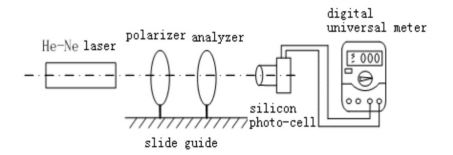
\includegraphics[width=0.9\textwidth]{Malu.jpg}
	\caption{Malus's Law}
	\label{fig1}
\end{figure}
Then we do the following three steps:
\begin{itemize}
    \item Rotate the analyzer for $360^\circ$ and observe the change in light intensity to find the maximum electric current \(I_0\).
    \item Set the angle of the analyzer to $90^\circ${} and adjust the angle of the polarizer until the electric current measured by the multimeter reaches its minimum. At this point, the polarizing axes of the polarizer and the analyzer are perpendicular to each other.
    \item Rotate the analyzer from $90^\circ${} to $0^\circ${} and record the magnitude of the current \(I\) every $5^\circ$. Record the values in a table and plot the graph of \(I / I_0\) versus \(\cos^2(\theta)\). Perform linear fitting and compare the data with the theoretical result.
\end{itemize}

\subsection{Linearly Polarized Light and the Half-wave Plate}
\indent

For this part of the experiment, we will do the following steps:
\begin{enumerate}
    \item Set up the equipment on the optical bench as shown in Figure 2.
    \begin{itemize}
        \item \textbf{A} is the analyzer, and \textbf{P} is the polarizer.
        \item Set the polarizing axes of \textbf{A} and \textbf{P} perpendicular to each other before placing the 1/2-wave plate in the apparatus; extinction of the light can be observed on the screen.
    \end{itemize}
    \item After inserting the 1/2-wave plate, rotate it to make the light extinction appear again and set this position as the initial position.
    \item Rotate the 1/2-wave plate for $\theta = 10^\circ$ from the initial position and the light extinction will be broken. Then rotate \textbf{A} to make the light extinction appear again, record the angle of rotation $\theta$ in a table.
    \item Rotate the 1/2-wave plate for $\theta = 20^\circ$ from the previous position (now $\theta = 20^\circ$) and repeat Step 3. Repeat this step (increase $\theta$) for 8 times. Plot the graph of $\theta$ versus the corresponding angle of the analyzer.
\end{enumerate}

\begin{figure}
	\centering
	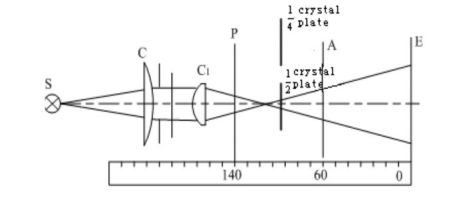
\includegraphics[width=0.9\textwidth]{TwoWave.jpg}
	\caption{Setup for 1/2 and 1/4-wave plates}
	\label{fig2}
\end{figure}

\subsection{Circularly and Elliptically Polarized Light and the 1/4-wave Plate}
\indent

For this part of the experiment, we will do the following steps:
\begin{enumerate}
    \item Set up the equipment on the optical bench as shown in Figure 2.
    \begin{itemize}
        \item \textbf{A} is the analyzer, and \textbf{P} is the polarizer.
        \item Set the polarizing axes of \textbf{A} and \textbf{P} perpendicular to each other before placing the 1/4-wave plate in the apparatus; extinction of the light can be observed on the screen. At this point, the angle $\theta = 90^\circ$.
    \end{itemize}
    \item After inserting the 1/4-wave plate, rotate it to make the light extinction appear again and set this position as the initial position. At this point, $\theta = 0^\circ$. Rotate the 1/4-wave plate and observe the change in the light intensity.
    \item Rotate the analyzer for 360° and record the light intensity (which is indicated by the current \textbf{I}) for every 10°. Record the data in a table.
    \item Rotate the 1/4-wave plate for 20° and repeat Step 3.
    \item Rotate the 1/4-wave plate for 45° and repeat Step 3.
    \item Rotate the 1/4-wave plate for 70°. Then rotate the analyzer and record its position and the magnitude of the current when the light intensity reaches a maximum.
    \item Use a computer to plot the relation between the rotation angle of the analyzer and the light amplitude in polar coordinates. Normalize the amplitude by its maximum value. Mark the position recorded in Step 6 and compare it with the data recorded in Step 4.
    \item Compare the result of Step 5 with that for the circular polarization. Plot a linear fit to the data when the angle is 45°.
\end{enumerate}

\section{Measurements and Results}
\subsection{Malus's Law}
\indent

We will apply an important equation for the demonstration of the Malus's Law:
\begin{equation*}
	I = I_0 \cos^2(\theta)
\end{equation*}
where \(I\) is the intensity of the light after passing through the analyzer, \(I_0\) is the maximum intensity of the light, and \(\theta\) is the angle between the polarizing axes of the polarizer and the analyzer.
The original data and plotted is shown as following with name of Figure 3 and 4
\begin{figure}
	\centering
	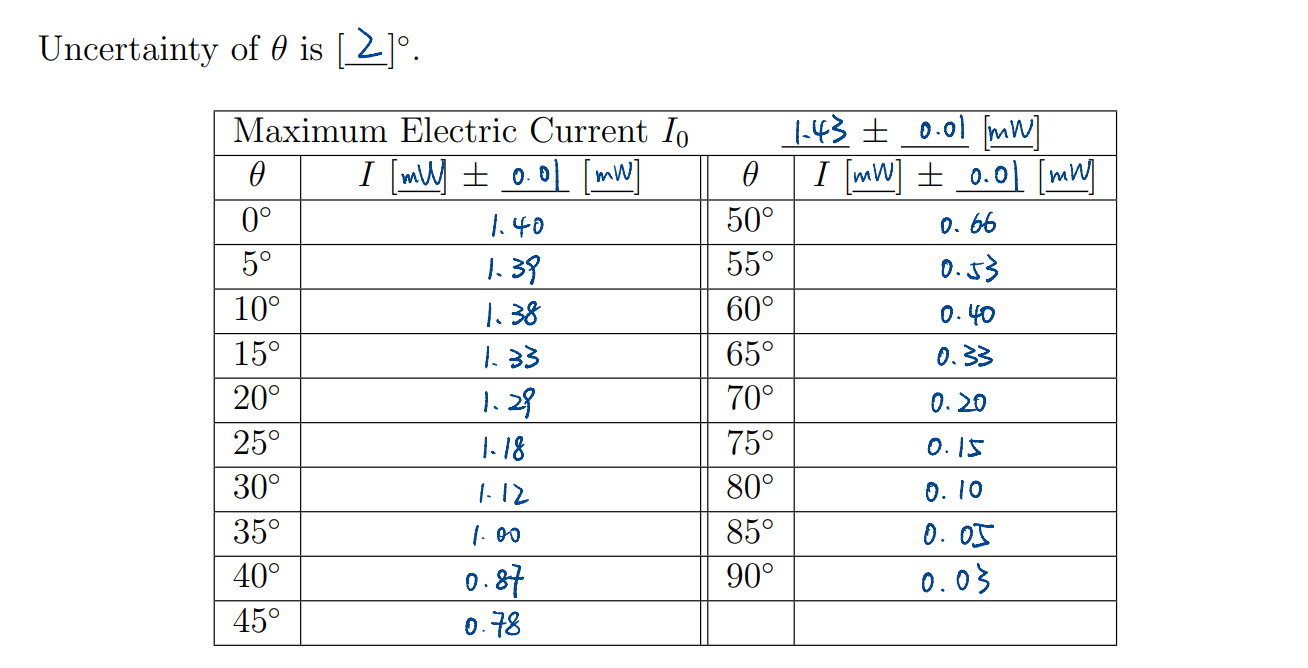
\includegraphics[width=0.9\textwidth]{Malu_Data.png}
	\caption{Malus's Law}
	\label{fig3}
\end{figure}
\begin{figure}
	\centering
	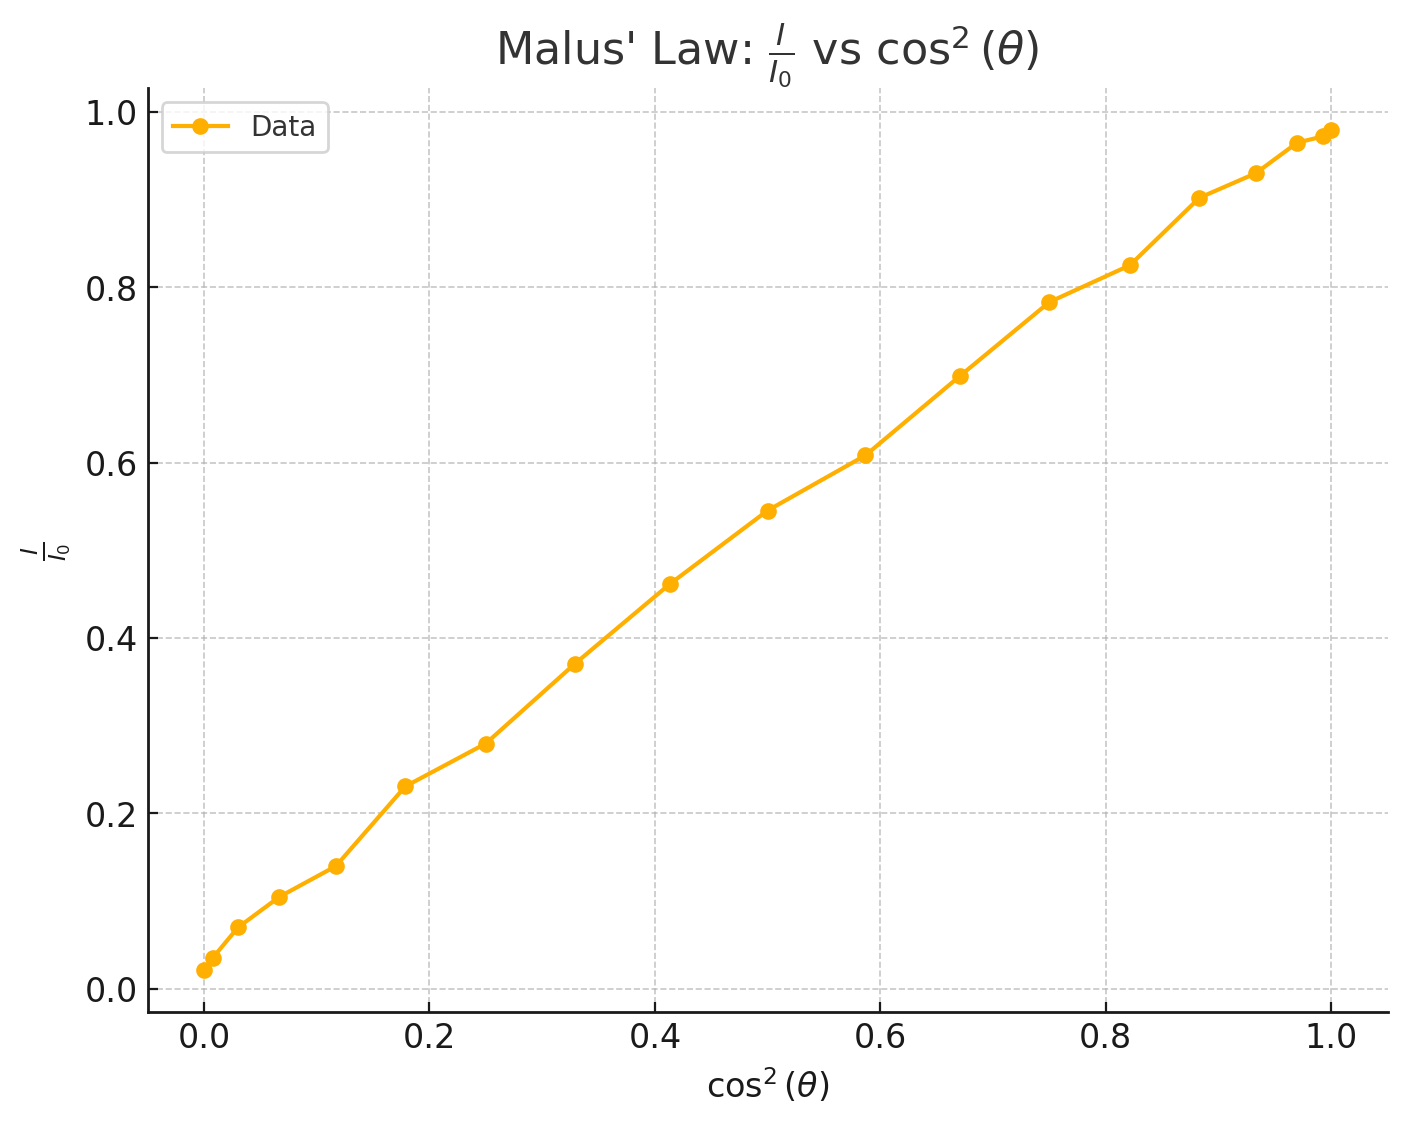
\includegraphics[width=0.9\textwidth]{Malu_Result.png}
	\caption{Malus's Law}
	\label{fig3}
\end{figure}

From the figure we can see that the value of $\frac{I}{I_0}$ is proportional to $\cos^2(\theta)$, which is consistent with the theoretical prediction. This should help
demonstrate the Malus's Law as mentioned above. 

\subsection{Linearly Polarized Light and the Half-wave Plate}
\indent

In this measurement part, we are looking at the relationship between the rotation angle of 1/2-wave plate and the angle of the analyzer. The original data and plotted is shown as following with name of Figure 5 and 6.
\begin{figure}
	\centering
	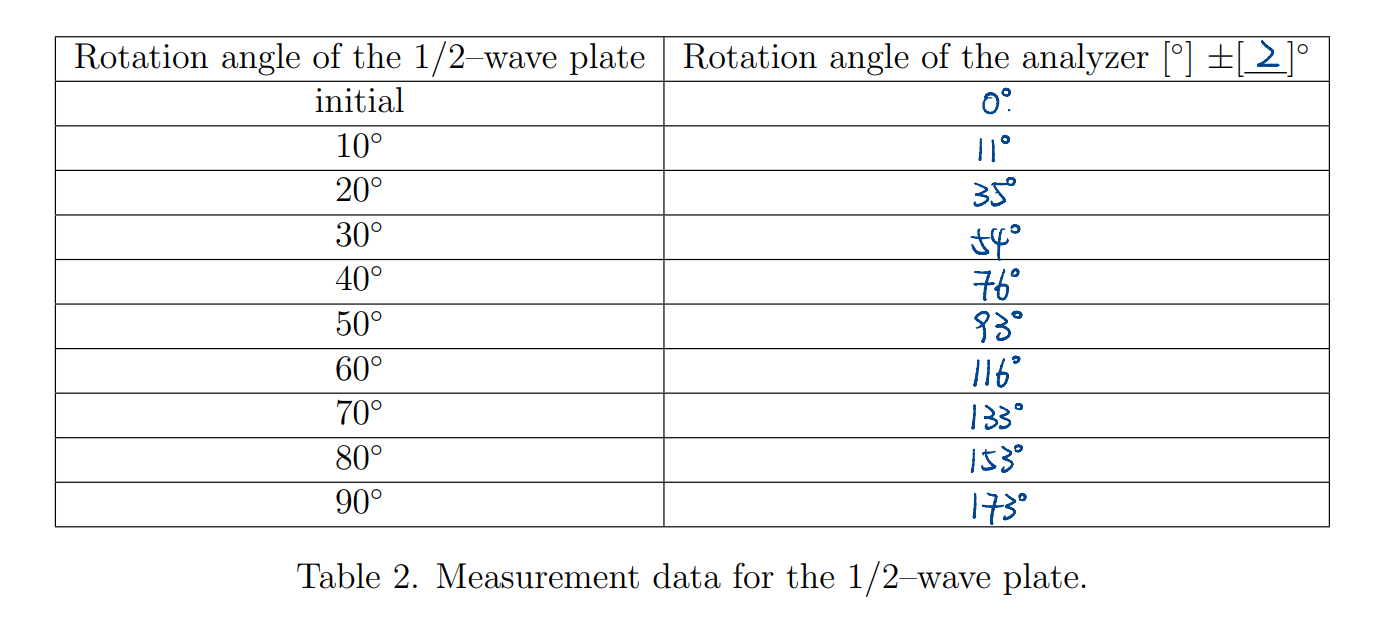
\includegraphics[width=0.9\textwidth]{HalfWave_Data.png}
	\caption{Half-wave plate}
	\label{fig5}
\end{figure}
\begin{figure}
	\centering
	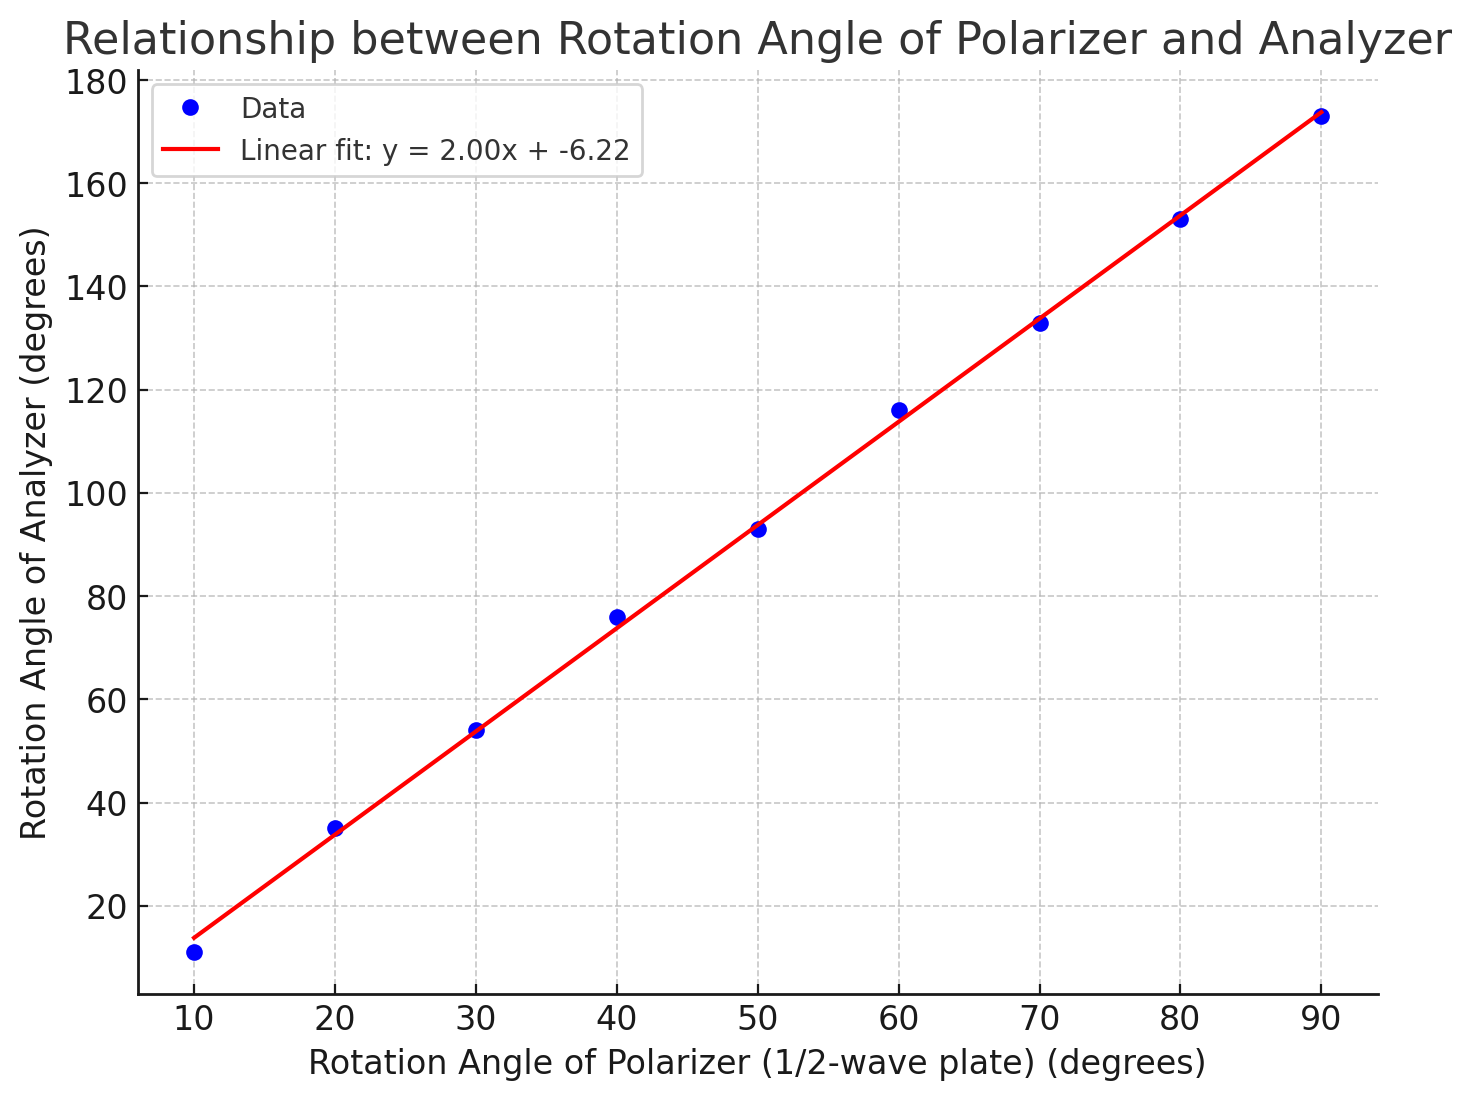
\includegraphics[width=0.9\textwidth]{HalfWave_Result.png}
	\caption{Half-wave plate}
	\label{fig6}
\end{figure}
From the plotted data we can see that the two sets of data are linearly related. The slope of the line is close to 2, which means that the rotation angle of the analyzer is 2 times the rotation angle of the 1/2-wave plate. 
This indicates that the polarization axis get rotated by twice of the origin angle(2$\alpha$) after the light passes through the 1/2-wave plate.

\subsection{Circularly and Elliptically Polarized Light and the 1/4-wave Plate}
\indent

There are three different experiments in this part. The first one is to observe the light intensity when the 1/4-wave plate is not rotated. 
The second is when the 1/4-wave plate is rotated by 20°. The third is when the 1/4-wave plate is rotated by 45°.
Since the original data takes too much space, we will just display them in the appendix. The plotted data is shown as following with name of Figure 7:
\begin{figure}
	\centering
	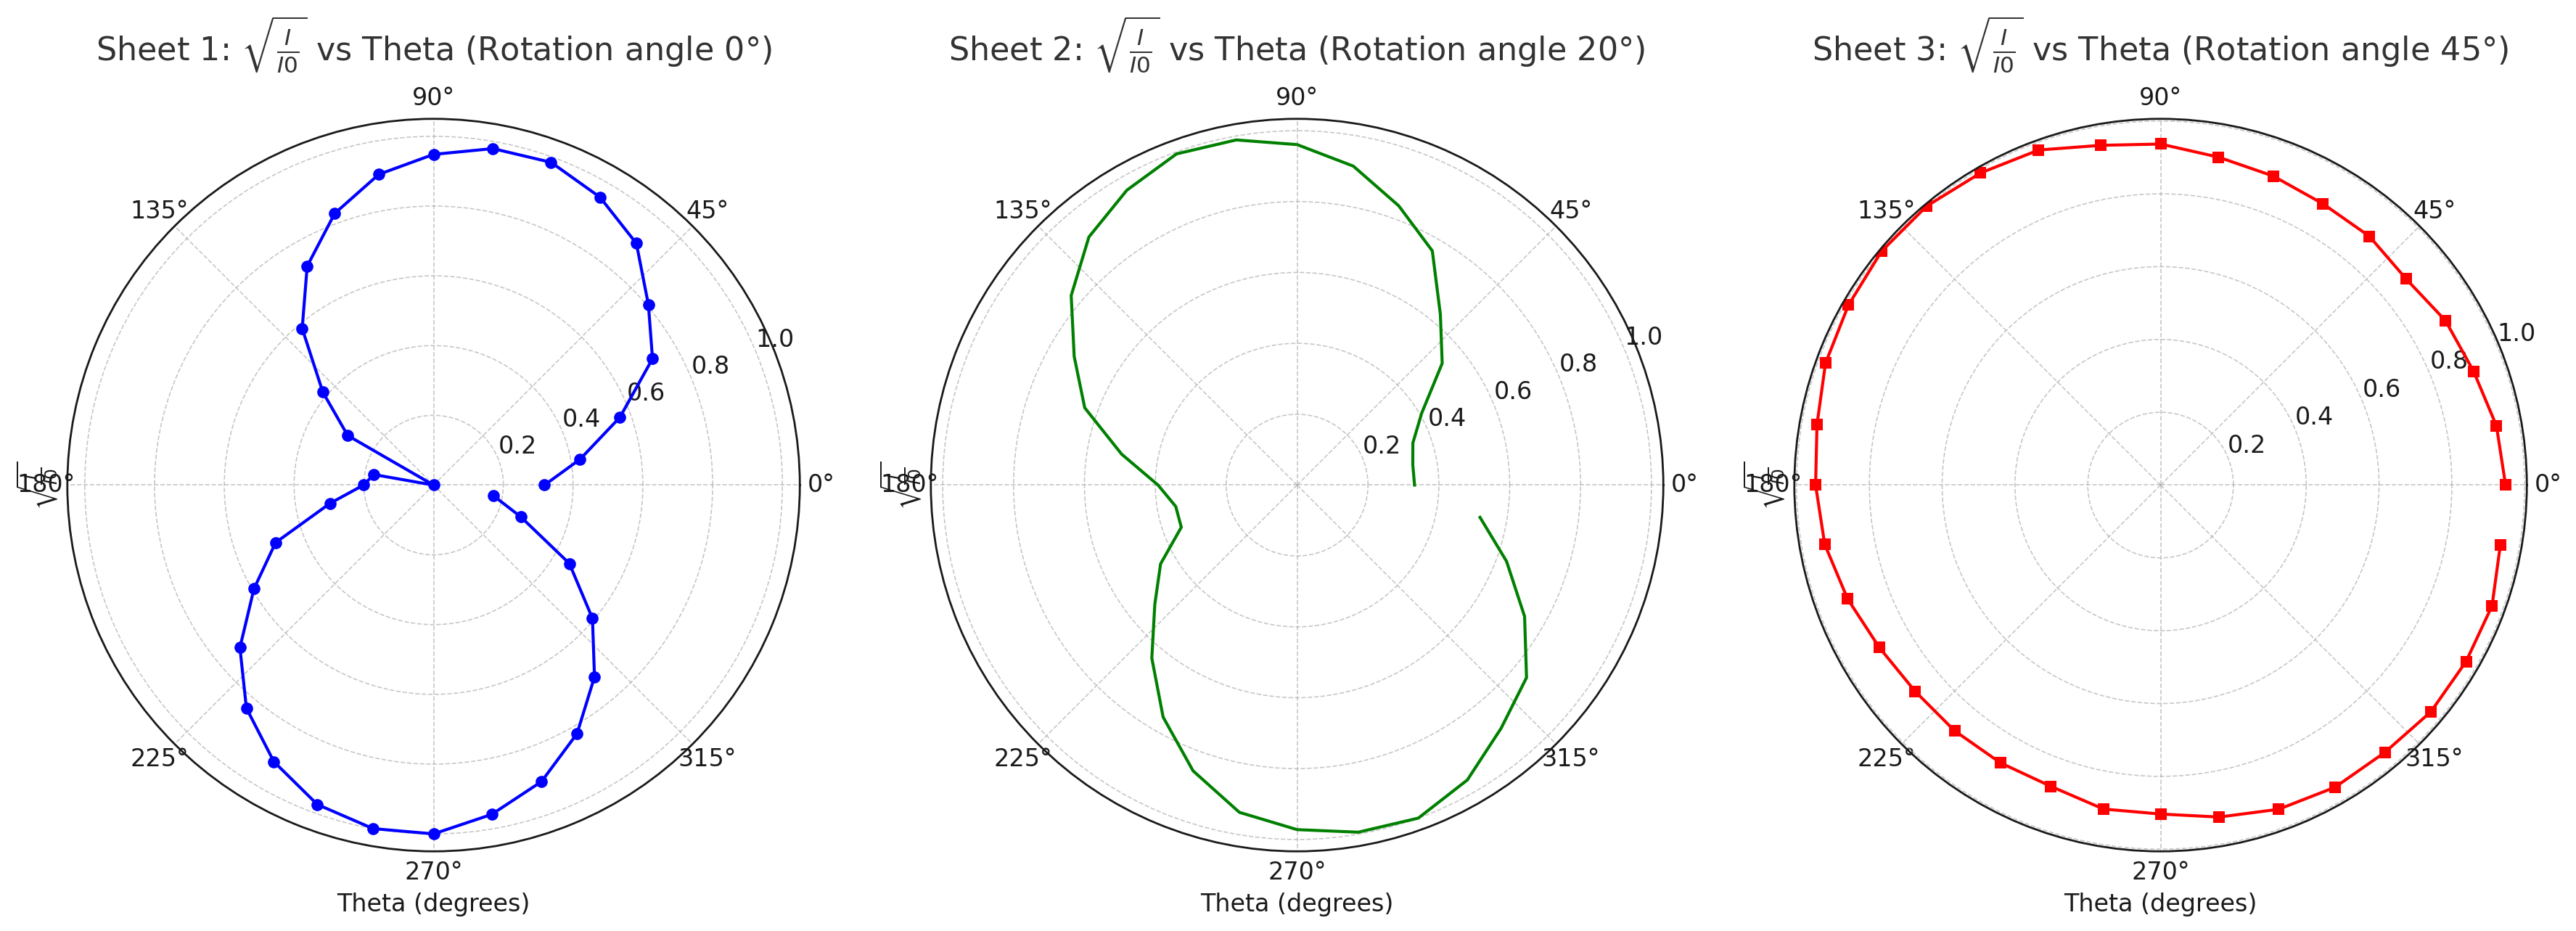
\includegraphics[width=0.9\textwidth]{QuarterWave_Result.png}
	\caption{Quarter-wave plate}
	\label{fig7}
\end{figure} 
From the plotted graph, we may draw some conclusions:
\begin{itemize}
	\item When the rotation angle of the 1/4 wave plate is $0^\circ$, the maximal light intensity is observed at about 90 and 270 degrees. Also from the figure we may see that the light source is linearly polarized.
	\item When the rotation angle of the 1/4 wave plate is $20^\circ$, the maximal light intensity is observed at about 110 and 290 degrees. The light source is elliptically polarized.
	\item When the rotation angle of the 1/4 wave plate is $45^\circ$, the maximal light intensity is observed at about 135 and 315 degrees. The light source is circularly polarized.
\end{itemize}
All the results are consistent with the theoretical prediction.

\section{Conclusions and discussion}
\subsection{Conclusions}
\indent

In this experiment, we have studied the polarization of light and the Malus's Law. We have also looked into the relationship between the intensity of light and the angle of the polarizer.
We discovered the different physical behavior when the light source goes through the half- and quarter-wave plates, and the corresponding polarization states of the light source. 
From the data we have collected, we have verified the Malus's Law and the theoretical prediction of the half- and quarter-wave plates. 

\subsection{Discussion}
\indent

Compared to the sample graph given, there are some discrepancies in the data we have collected. The mistakes may have been caused by various reasons:
\begin{itemize}
	\item The light source may not be perfectly linearly polarized, which may lead to some errors in the data.
	\item The angle of the polarizer and the analyzer may have some errors in rotation, which cause mistakes.
	\item The equipment may not be perfectly calibrated due to long terms of use, which may lead to some errors in the data.
\end{itemize}
Here are some possible improvements to the experiment:
\begin{itemize}
	\item Use a more stable light source to ensure the light is linearly polarized.
	\item Use a more precise device to measure the angle of the polarizer and the analyzer.
	\item Calibrate the equipment more frequently to ensure the accuracy of the data.
\end{itemize}

\section{Works cited}
Department of Physics, Shanghai Jiaotong University, Exercise 4 (Polarization of Light) - lab manual [rev. 2.8], 2024\\
Python Software Foundation. (2020). Python Language Reference, version 3.9. Available at http://www.python.org\\
\\
All the figures displayed in the article (excluding the appendix) are given using Python 3.9.
\pagebreak
\appendix
\section{Datasheet}
\begin{figure}
	\centering
	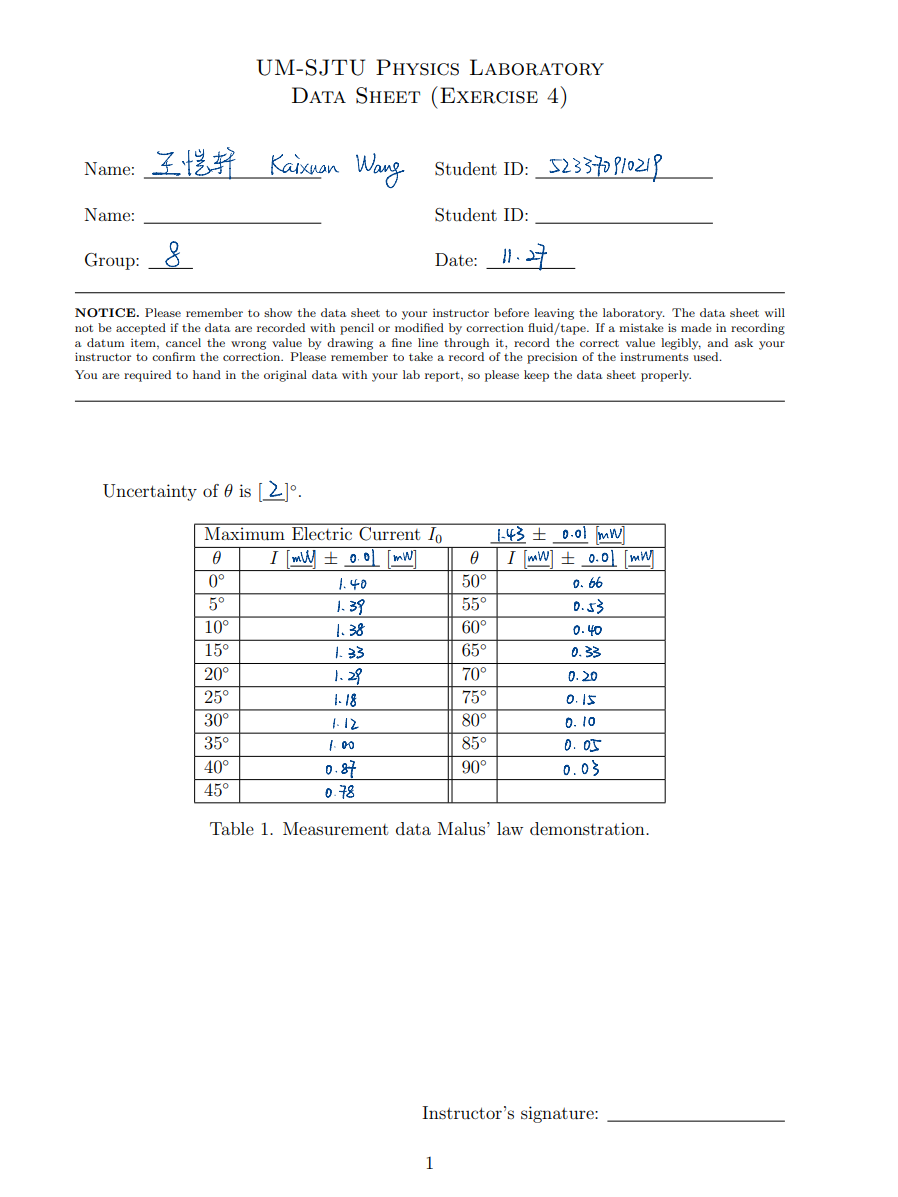
\includegraphics[width=0.9\textwidth]{D1.png}
	\label{fig8}
\end{figure}

\begin{figure}
	\centering
	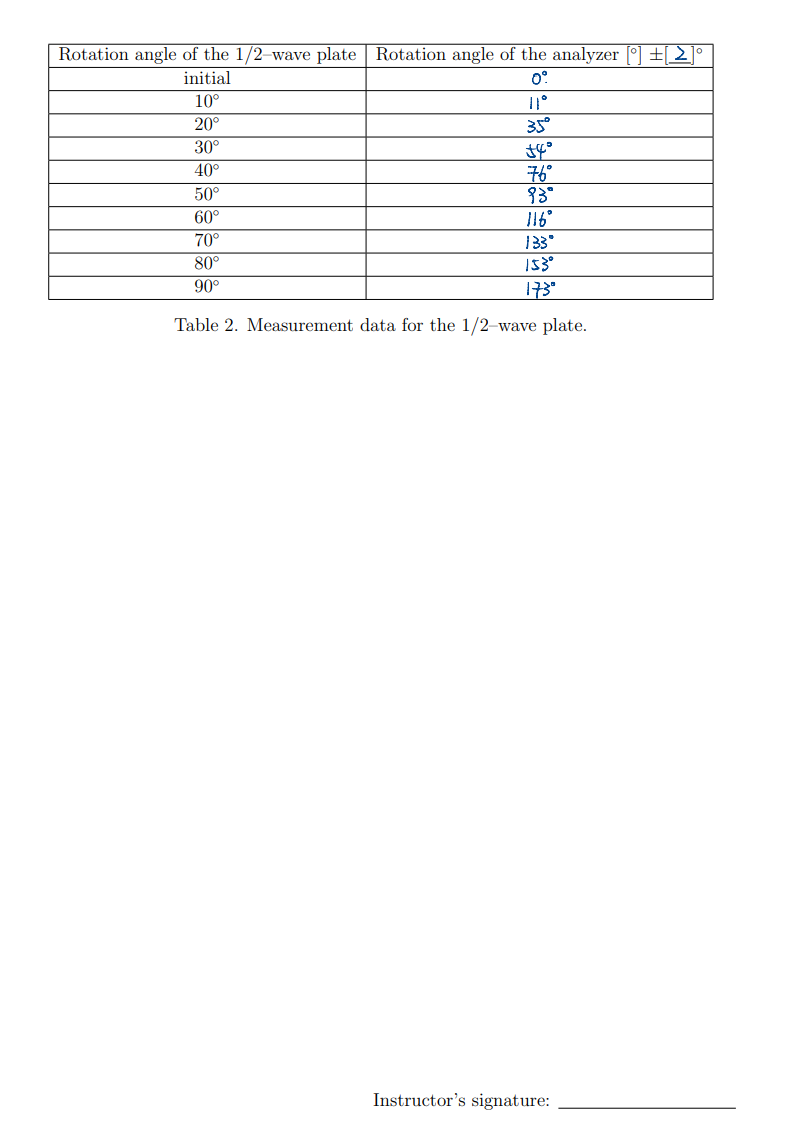
\includegraphics[width=0.9\textwidth]{D2.png}
	\label{fig9}
\end{figure}

\begin{figure}
	\centering
	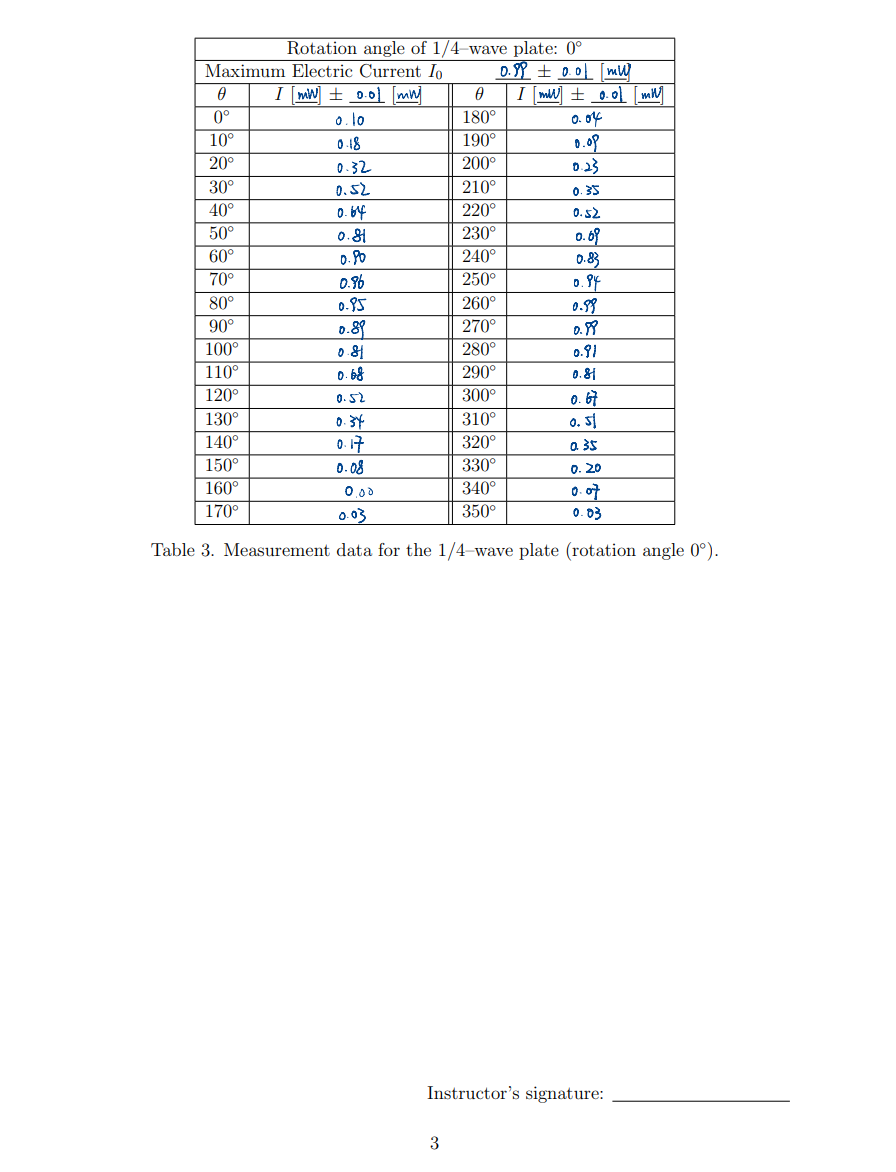
\includegraphics[width=0.9\textwidth]{D3.png}
	\label{fig10}
\end{figure}

\begin{figure}
	\centering
	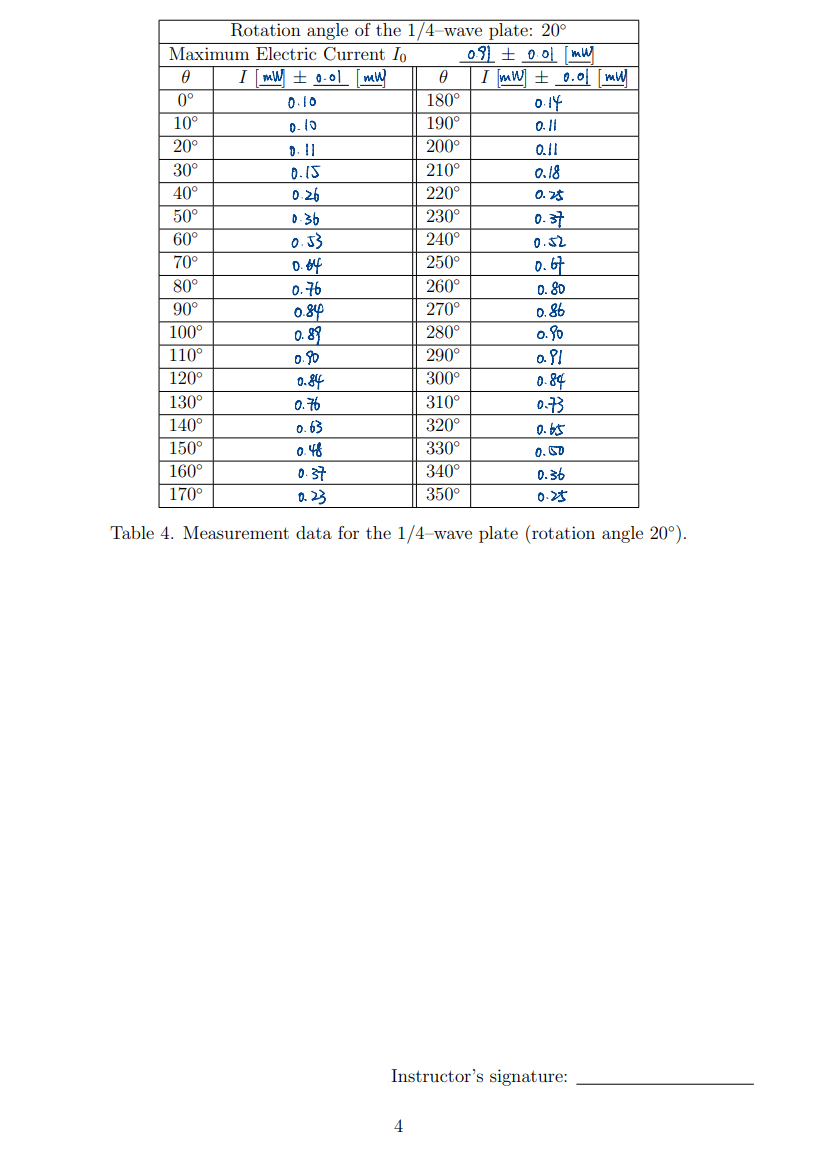
\includegraphics[width=0.9\textwidth]{D4.png}
	\label{fig11}
\end{figure}

\begin{figure}
	\centering
	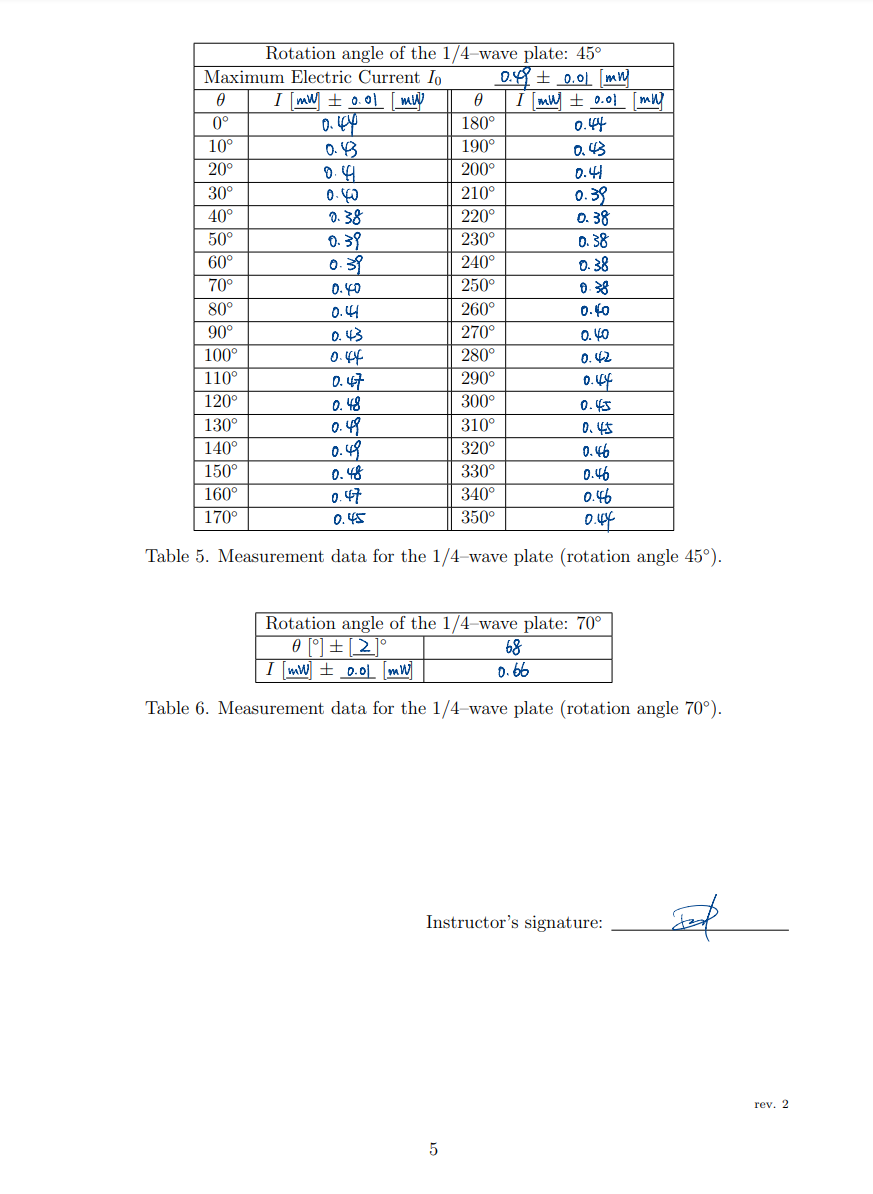
\includegraphics[width=0.9\textwidth]{D5.png}
	\label{fig12}
\end{figure}


%\textcolor{blue}{Please remember to attach the original data sheet signed by your instructor.}
\end{document}